% Options for packages loaded elsewhere
% Options for packages loaded elsewhere
\PassOptionsToPackage{unicode}{hyperref}
\PassOptionsToPackage{hyphens}{url}
\PassOptionsToPackage{dvipsnames,svgnames,x11names}{xcolor}
%
\documentclass[
  letterpaper,
  DIV=11,
  numbers=noendperiod]{scrreprt}
\usepackage{xcolor}
\usepackage{amsmath,amssymb}
\setcounter{secnumdepth}{5}
\usepackage{iftex}
\ifPDFTeX
  \usepackage[T1]{fontenc}
  \usepackage[utf8]{inputenc}
  \usepackage{textcomp} % provide euro and other symbols
\else % if luatex or xetex
  \usepackage{unicode-math} % this also loads fontspec
  \defaultfontfeatures{Scale=MatchLowercase}
  \defaultfontfeatures[\rmfamily]{Ligatures=TeX,Scale=1}
\fi
\usepackage{lmodern}
\ifPDFTeX\else
  % xetex/luatex font selection
\fi
% Use upquote if available, for straight quotes in verbatim environments
\IfFileExists{upquote.sty}{\usepackage{upquote}}{}
\IfFileExists{microtype.sty}{% use microtype if available
  \usepackage[]{microtype}
  \UseMicrotypeSet[protrusion]{basicmath} % disable protrusion for tt fonts
}{}
\makeatletter
\@ifundefined{KOMAClassName}{% if non-KOMA class
  \IfFileExists{parskip.sty}{%
    \usepackage{parskip}
  }{% else
    \setlength{\parindent}{0pt}
    \setlength{\parskip}{6pt plus 2pt minus 1pt}}
}{% if KOMA class
  \KOMAoptions{parskip=half}}
\makeatother
% Make \paragraph and \subparagraph free-standing
\makeatletter
\ifx\paragraph\undefined\else
  \let\oldparagraph\paragraph
  \renewcommand{\paragraph}{
    \@ifstar
      \xxxParagraphStar
      \xxxParagraphNoStar
  }
  \newcommand{\xxxParagraphStar}[1]{\oldparagraph*{#1}\mbox{}}
  \newcommand{\xxxParagraphNoStar}[1]{\oldparagraph{#1}\mbox{}}
\fi
\ifx\subparagraph\undefined\else
  \let\oldsubparagraph\subparagraph
  \renewcommand{\subparagraph}{
    \@ifstar
      \xxxSubParagraphStar
      \xxxSubParagraphNoStar
  }
  \newcommand{\xxxSubParagraphStar}[1]{\oldsubparagraph*{#1}\mbox{}}
  \newcommand{\xxxSubParagraphNoStar}[1]{\oldsubparagraph{#1}\mbox{}}
\fi
\makeatother

\usepackage{color}
\usepackage{fancyvrb}
\newcommand{\VerbBar}{|}
\newcommand{\VERB}{\Verb[commandchars=\\\{\}]}
\DefineVerbatimEnvironment{Highlighting}{Verbatim}{commandchars=\\\{\}}
% Add ',fontsize=\small' for more characters per line
\usepackage{framed}
\definecolor{shadecolor}{RGB}{241,243,245}
\newenvironment{Shaded}{\begin{snugshade}}{\end{snugshade}}
\newcommand{\AlertTok}[1]{\textcolor[rgb]{0.68,0.00,0.00}{#1}}
\newcommand{\AnnotationTok}[1]{\textcolor[rgb]{0.37,0.37,0.37}{#1}}
\newcommand{\AttributeTok}[1]{\textcolor[rgb]{0.40,0.45,0.13}{#1}}
\newcommand{\BaseNTok}[1]{\textcolor[rgb]{0.68,0.00,0.00}{#1}}
\newcommand{\BuiltInTok}[1]{\textcolor[rgb]{0.00,0.23,0.31}{#1}}
\newcommand{\CharTok}[1]{\textcolor[rgb]{0.13,0.47,0.30}{#1}}
\newcommand{\CommentTok}[1]{\textcolor[rgb]{0.37,0.37,0.37}{#1}}
\newcommand{\CommentVarTok}[1]{\textcolor[rgb]{0.37,0.37,0.37}{\textit{#1}}}
\newcommand{\ConstantTok}[1]{\textcolor[rgb]{0.56,0.35,0.01}{#1}}
\newcommand{\ControlFlowTok}[1]{\textcolor[rgb]{0.00,0.23,0.31}{\textbf{#1}}}
\newcommand{\DataTypeTok}[1]{\textcolor[rgb]{0.68,0.00,0.00}{#1}}
\newcommand{\DecValTok}[1]{\textcolor[rgb]{0.68,0.00,0.00}{#1}}
\newcommand{\DocumentationTok}[1]{\textcolor[rgb]{0.37,0.37,0.37}{\textit{#1}}}
\newcommand{\ErrorTok}[1]{\textcolor[rgb]{0.68,0.00,0.00}{#1}}
\newcommand{\ExtensionTok}[1]{\textcolor[rgb]{0.00,0.23,0.31}{#1}}
\newcommand{\FloatTok}[1]{\textcolor[rgb]{0.68,0.00,0.00}{#1}}
\newcommand{\FunctionTok}[1]{\textcolor[rgb]{0.28,0.35,0.67}{#1}}
\newcommand{\ImportTok}[1]{\textcolor[rgb]{0.00,0.46,0.62}{#1}}
\newcommand{\InformationTok}[1]{\textcolor[rgb]{0.37,0.37,0.37}{#1}}
\newcommand{\KeywordTok}[1]{\textcolor[rgb]{0.00,0.23,0.31}{\textbf{#1}}}
\newcommand{\NormalTok}[1]{\textcolor[rgb]{0.00,0.23,0.31}{#1}}
\newcommand{\OperatorTok}[1]{\textcolor[rgb]{0.37,0.37,0.37}{#1}}
\newcommand{\OtherTok}[1]{\textcolor[rgb]{0.00,0.23,0.31}{#1}}
\newcommand{\PreprocessorTok}[1]{\textcolor[rgb]{0.68,0.00,0.00}{#1}}
\newcommand{\RegionMarkerTok}[1]{\textcolor[rgb]{0.00,0.23,0.31}{#1}}
\newcommand{\SpecialCharTok}[1]{\textcolor[rgb]{0.37,0.37,0.37}{#1}}
\newcommand{\SpecialStringTok}[1]{\textcolor[rgb]{0.13,0.47,0.30}{#1}}
\newcommand{\StringTok}[1]{\textcolor[rgb]{0.13,0.47,0.30}{#1}}
\newcommand{\VariableTok}[1]{\textcolor[rgb]{0.07,0.07,0.07}{#1}}
\newcommand{\VerbatimStringTok}[1]{\textcolor[rgb]{0.13,0.47,0.30}{#1}}
\newcommand{\WarningTok}[1]{\textcolor[rgb]{0.37,0.37,0.37}{\textit{#1}}}

\usepackage{longtable,booktabs,array}
\usepackage{calc} % for calculating minipage widths
% Correct order of tables after \paragraph or \subparagraph
\usepackage{etoolbox}
\makeatletter
\patchcmd\longtable{\par}{\if@noskipsec\mbox{}\fi\par}{}{}
\makeatother
% Allow footnotes in longtable head/foot
\IfFileExists{footnotehyper.sty}{\usepackage{footnotehyper}}{\usepackage{footnote}}
\makesavenoteenv{longtable}
\usepackage{graphicx}
\makeatletter
\newsavebox\pandoc@box
\newcommand*\pandocbounded[1]{% scales image to fit in text height/width
  \sbox\pandoc@box{#1}%
  \Gscale@div\@tempa{\textheight}{\dimexpr\ht\pandoc@box+\dp\pandoc@box\relax}%
  \Gscale@div\@tempb{\linewidth}{\wd\pandoc@box}%
  \ifdim\@tempb\p@<\@tempa\p@\let\@tempa\@tempb\fi% select the smaller of both
  \ifdim\@tempa\p@<\p@\scalebox{\@tempa}{\usebox\pandoc@box}%
  \else\usebox{\pandoc@box}%
  \fi%
}
% Set default figure placement to htbp
\def\fps@figure{htbp}
\makeatother





\setlength{\emergencystretch}{3em} % prevent overfull lines

\providecommand{\tightlist}{%
  \setlength{\itemsep}{0pt}\setlength{\parskip}{0pt}}



 


\KOMAoption{captions}{tableheading}
\makeatletter
\@ifpackageloaded{tcolorbox}{}{\usepackage[skins,breakable]{tcolorbox}}
\@ifpackageloaded{fontawesome5}{}{\usepackage{fontawesome5}}
\definecolor{quarto-callout-color}{HTML}{909090}
\definecolor{quarto-callout-note-color}{HTML}{0758E5}
\definecolor{quarto-callout-important-color}{HTML}{CC1914}
\definecolor{quarto-callout-warning-color}{HTML}{EB9113}
\definecolor{quarto-callout-tip-color}{HTML}{00A047}
\definecolor{quarto-callout-caution-color}{HTML}{FC5300}
\definecolor{quarto-callout-color-frame}{HTML}{acacac}
\definecolor{quarto-callout-note-color-frame}{HTML}{4582ec}
\definecolor{quarto-callout-important-color-frame}{HTML}{d9534f}
\definecolor{quarto-callout-warning-color-frame}{HTML}{f0ad4e}
\definecolor{quarto-callout-tip-color-frame}{HTML}{02b875}
\definecolor{quarto-callout-caution-color-frame}{HTML}{fd7e14}
\makeatother
\makeatletter
\@ifpackageloaded{bookmark}{}{\usepackage{bookmark}}
\makeatother
\makeatletter
\@ifpackageloaded{caption}{}{\usepackage{caption}}
\AtBeginDocument{%
\ifdefined\contentsname
  \renewcommand*\contentsname{Table of contents}
\else
  \newcommand\contentsname{Table of contents}
\fi
\ifdefined\listfigurename
  \renewcommand*\listfigurename{List of Figures}
\else
  \newcommand\listfigurename{List of Figures}
\fi
\ifdefined\listtablename
  \renewcommand*\listtablename{List of Tables}
\else
  \newcommand\listtablename{List of Tables}
\fi
\ifdefined\figurename
  \renewcommand*\figurename{Figure}
\else
  \newcommand\figurename{Figure}
\fi
\ifdefined\tablename
  \renewcommand*\tablename{Table}
\else
  \newcommand\tablename{Table}
\fi
}
\@ifpackageloaded{float}{}{\usepackage{float}}
\floatstyle{ruled}
\@ifundefined{c@chapter}{\newfloat{codelisting}{h}{lop}}{\newfloat{codelisting}{h}{lop}[chapter]}
\floatname{codelisting}{Listing}
\newcommand*\listoflistings{\listof{codelisting}{List of Listings}}
\makeatother
\makeatletter
\makeatother
\makeatletter
\@ifpackageloaded{caption}{}{\usepackage{caption}}
\@ifpackageloaded{subcaption}{}{\usepackage{subcaption}}
\makeatother
\usepackage{bookmark}
\IfFileExists{xurl.sty}{\usepackage{xurl}}{} % add URL line breaks if available
\urlstyle{same}
\hypersetup{
  pdftitle={Pip Technical Guidelines},
  pdfauthor={R.Andres Castenada; Ronak Shah},
  colorlinks=true,
  linkcolor={blue},
  filecolor={Maroon},
  citecolor={Blue},
  urlcolor={Blue},
  pdfcreator={LaTeX via pandoc}}


\title{Pip Technical Guidelines}
\author{R.Andres Castenada \and Ronak Shah}
\date{2025-08-03}
\begin{document}
\maketitle

\renewcommand*\contentsname{Table of contents}
{
\hypersetup{linkcolor=}
\setcounter{tocdepth}{2}
\tableofcontents
}

\bookmarksetup{startatroot}

\chapter*{Preface}\label{preface}
\addcontentsline{toc}{chapter}{Preface}

\markboth{Preface}{Preface}

This is a Quarto book. In this book we intend to write technical
information about PIP projects.

\bookmarksetup{startatroot}

\chapter{Introduction}\label{introduction}

The purpose of this book is to gather all the technical knowledge
specific to PIP in one place.

\bookmarksetup{startatroot}

\chapter{Add code coverage badge to your GitHub
Repository.}\label{add-code-coverage-badge-to-your-github-repository.}

In this article we will learn how to add code coverage badge to your
GitHub repository.

\section{Codecov.io}\label{codecov.io}

\begin{itemize}
\item
  Create an account at \url{https://about.codecov.io/} , sign up with
  your GitHub account if you don't have an account already.
  \textbf{Codecov} is a popular tool for measuring and visualizing
  \textbf{code coverage} in software projects. It integrates with
  GitHub, GitLab, Bitbucket, and other CI/CD systems to provide insights
  into how much of your code is tested by your test suite.
\item
  You can sync your private Github repositories on codecov platform to
  get started. If you want to add code coverage badge to a repository
  which is part of an organization (like PIP-Technical-Team, GPID-WB
  etc) then you need to be an admin of that organization. Admin role is
  needed because to sync the communication between Codecov.io with
  GitHub we need to generate a token which can only be done by admins.
\item
  Once your repo is synced with codecov and you can see it there click
  on Configure to start the process. As an example it should give you
  this screen
\end{itemize}

\pandocbounded{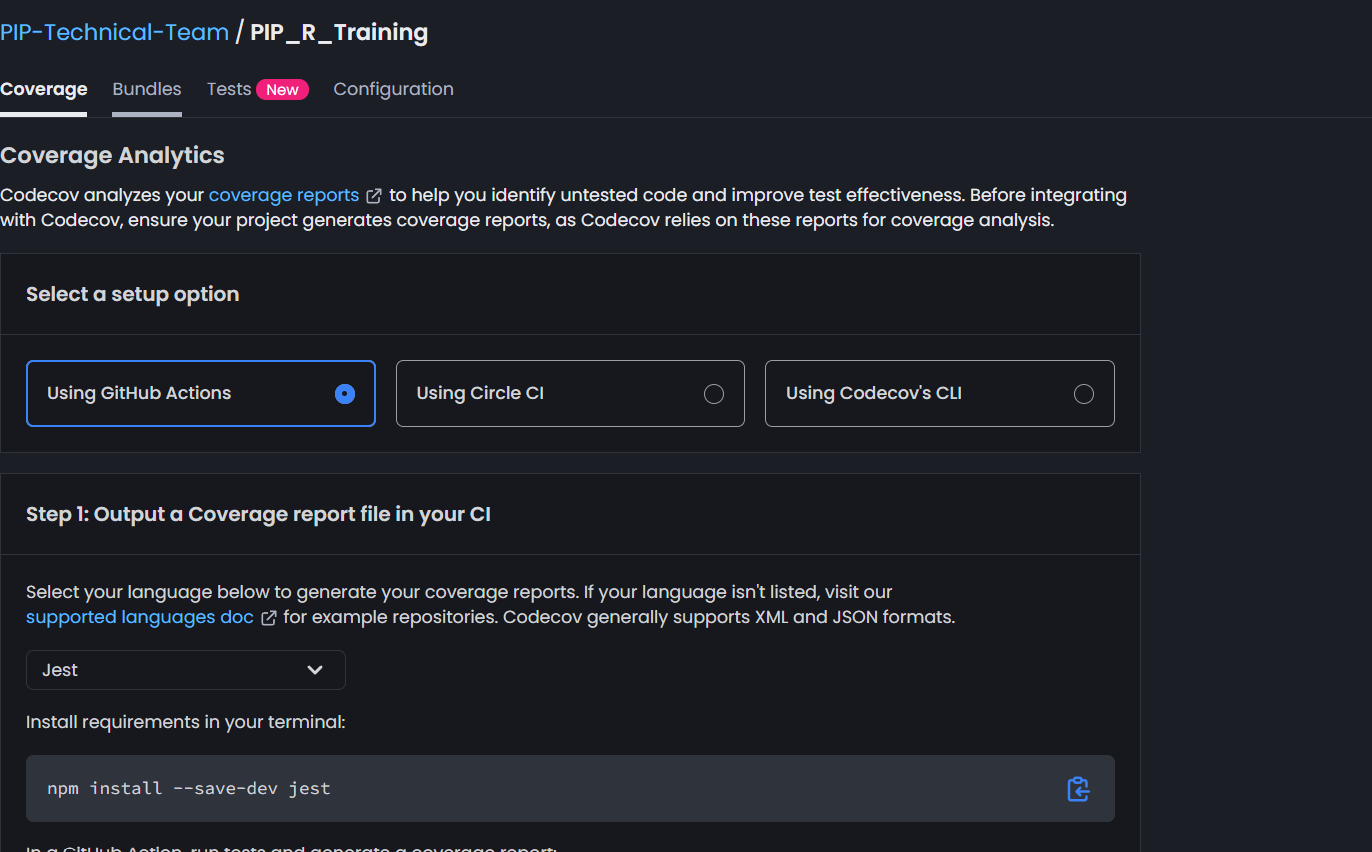
\includegraphics[keepaspectratio]{images/clipboard-644830120.png}}

\begin{itemize}
\item
  If you scroll below it will ask you to generate a repository secret,
  click on that to get a unique token for your repository and copy it.
\item
  You can ignore rest of the steps mentioned on that page since those
  are very generic language agnostic steps and since we want to setup
  this for R packages, we have a better option which I will share below.
\end{itemize}

\section{GitHub}\label{github}

\begin{itemize}
\item
  Now, moving to GitHub go to your repository. Click on Settings
  -\textgreater{} Secrets and Variables -\textgreater{} Actions
  -\textgreater{} Repository Secrets add the new token with name
  \texttt{CODECOV\_TOKEN} and copy the token value which was generated
  in the previous step.

  \pandocbounded{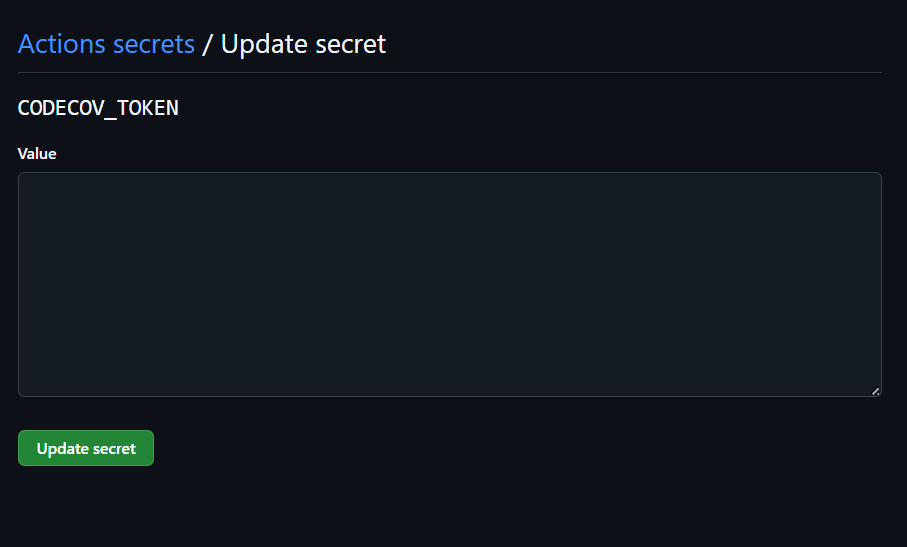
\includegraphics[keepaspectratio]{images/clipboard-1807060945.png}}
\item
  Next, we are going to setup GitHub Action to run and calculate code
  coverage after every push. The calculated coverage report would be
  uploaded on codecov.io and would be visible on their dashboard.
\item
  Additionally, I also added a possibility to run \texttt{R\ CMD\ CHECK}
  after every push. \texttt{R\ CMD\ check} is a tool that runs a series
  of automated checks on an R package to ensure it's correctly
  structured, documented, and error-free. It helps catch issues in code,
  tests, and documentation before sharing or submitting to CRAN. So it
  is like an additional validation that we have on our code.
\item
  The new workflow file looks like below

\begin{Shaded}
\begin{Highlighting}[]
\FunctionTok{name}\KeywordTok{:}\AttributeTok{ R{-}CMD{-}check and Codecov}

\FunctionTok{on}\KeywordTok{:}
\AttributeTok{  }\FunctionTok{push}\KeywordTok{:}
\AttributeTok{    }\FunctionTok{branches}\KeywordTok{:}\AttributeTok{ }\KeywordTok{[}\AttributeTok{master}\KeywordTok{]}
\AttributeTok{  }\FunctionTok{pull\_request}\KeywordTok{:}
\AttributeTok{    }\FunctionTok{branches}\KeywordTok{:}\AttributeTok{ }\KeywordTok{[}\AttributeTok{master}\KeywordTok{]}

\FunctionTok{jobs}\KeywordTok{:}
\AttributeTok{  }\FunctionTok{R{-}CMD{-}check}\KeywordTok{:}
\AttributeTok{    }\FunctionTok{runs{-}on}\KeywordTok{:}\AttributeTok{ ubuntu{-}latest}

\AttributeTok{    }\FunctionTok{steps}\KeywordTok{:}
\AttributeTok{      }\KeywordTok{{-}}\AttributeTok{ }\FunctionTok{name}\KeywordTok{:}\AttributeTok{ Checkout repository}
\AttributeTok{        }\FunctionTok{uses}\KeywordTok{:}\AttributeTok{ actions/checkout@v4}

\AttributeTok{      }\KeywordTok{{-}}\AttributeTok{ }\FunctionTok{name}\KeywordTok{:}\AttributeTok{ Set up R}
\AttributeTok{        }\FunctionTok{uses}\KeywordTok{:}\AttributeTok{ r{-}lib/actions/setup{-}r@v2}

\AttributeTok{      }\KeywordTok{{-}}\AttributeTok{ }\FunctionTok{name}\KeywordTok{:}\AttributeTok{ Set up pandoc}
\AttributeTok{        }\FunctionTok{uses}\KeywordTok{:}\AttributeTok{ r{-}lib/actions/setup{-}pandoc@v2}

\AttributeTok{      }\KeywordTok{{-}}\AttributeTok{ }\FunctionTok{name}\KeywordTok{:}\AttributeTok{ Install dependencies}
\FunctionTok{        run}\KeywordTok{: }\CharTok{|}
\NormalTok{          install.packages(c("remotes", "rcmdcheck", "covr"))}
\NormalTok{          remotes::install\_deps(dependencies = TRUE)}
\AttributeTok{        }\FunctionTok{shell}\KeywordTok{:}\AttributeTok{ Rscript \{0\}}

\AttributeTok{      }\KeywordTok{{-}}\AttributeTok{ }\FunctionTok{name}\KeywordTok{:}\AttributeTok{ Run R CMD check}
\FunctionTok{        run}\KeywordTok{: }\CharTok{|}
\NormalTok{          rcmdcheck::rcmdcheck(args = "{-}{-}no{-}manual", error\_on = "warning")}
\AttributeTok{        }\FunctionTok{shell}\KeywordTok{:}\AttributeTok{ Rscript \{0\}}

\AttributeTok{      }\KeywordTok{{-}}\AttributeTok{ }\FunctionTok{name}\KeywordTok{:}\AttributeTok{ Run test coverage}
\FunctionTok{        run}\KeywordTok{: }\CharTok{|}
\NormalTok{          covr::codecov()}
\AttributeTok{        }\FunctionTok{shell}\KeywordTok{:}\AttributeTok{ Rscript \{0\}}
\AttributeTok{        }\FunctionTok{env}\KeywordTok{:}
\AttributeTok{          }\FunctionTok{CODECOV\_TOKEN}\KeywordTok{:}\AttributeTok{ $\{\{ secrets.CODECOV\_TOKEN \}\} }
\end{Highlighting}
\end{Shaded}
\item
  This file is self explanatory but briefly, it checks out the
  repository that we want to run our action on, sets up R to run
  \texttt{R\ CMD\ CHECK} and finally generate code coverage report and
  upload it to codecov.io .
\item
  One tip that I can share is to check if this workflow file works on
  your local branch before running on \texttt{master} branch. To do that
  you should temporarily enable the workflow file to run on your local
  branch. This can be done as below -

\begin{Shaded}
\begin{Highlighting}[]
\FunctionTok{on}\KeywordTok{:}
\AttributeTok{  }\FunctionTok{push}\KeywordTok{:}
\AttributeTok{    }\FunctionTok{branches}\KeywordTok{:}\AttributeTok{ }\KeywordTok{[}\AttributeTok{master}\KeywordTok{,}\AttributeTok{ your{-}branch}\KeywordTok{]}
\end{Highlighting}
\end{Shaded}

  where \texttt{your-branch} is the name of the local branch that you
  want to run the workflow for. Once you have verified that everything
  works as expected in the local branch, you can remove
  \texttt{your-branch} from the list again.
\item
  Once the workflow runs successfully the dashboard on codecov.io should
  be updated and you should see something like this

  \pandocbounded{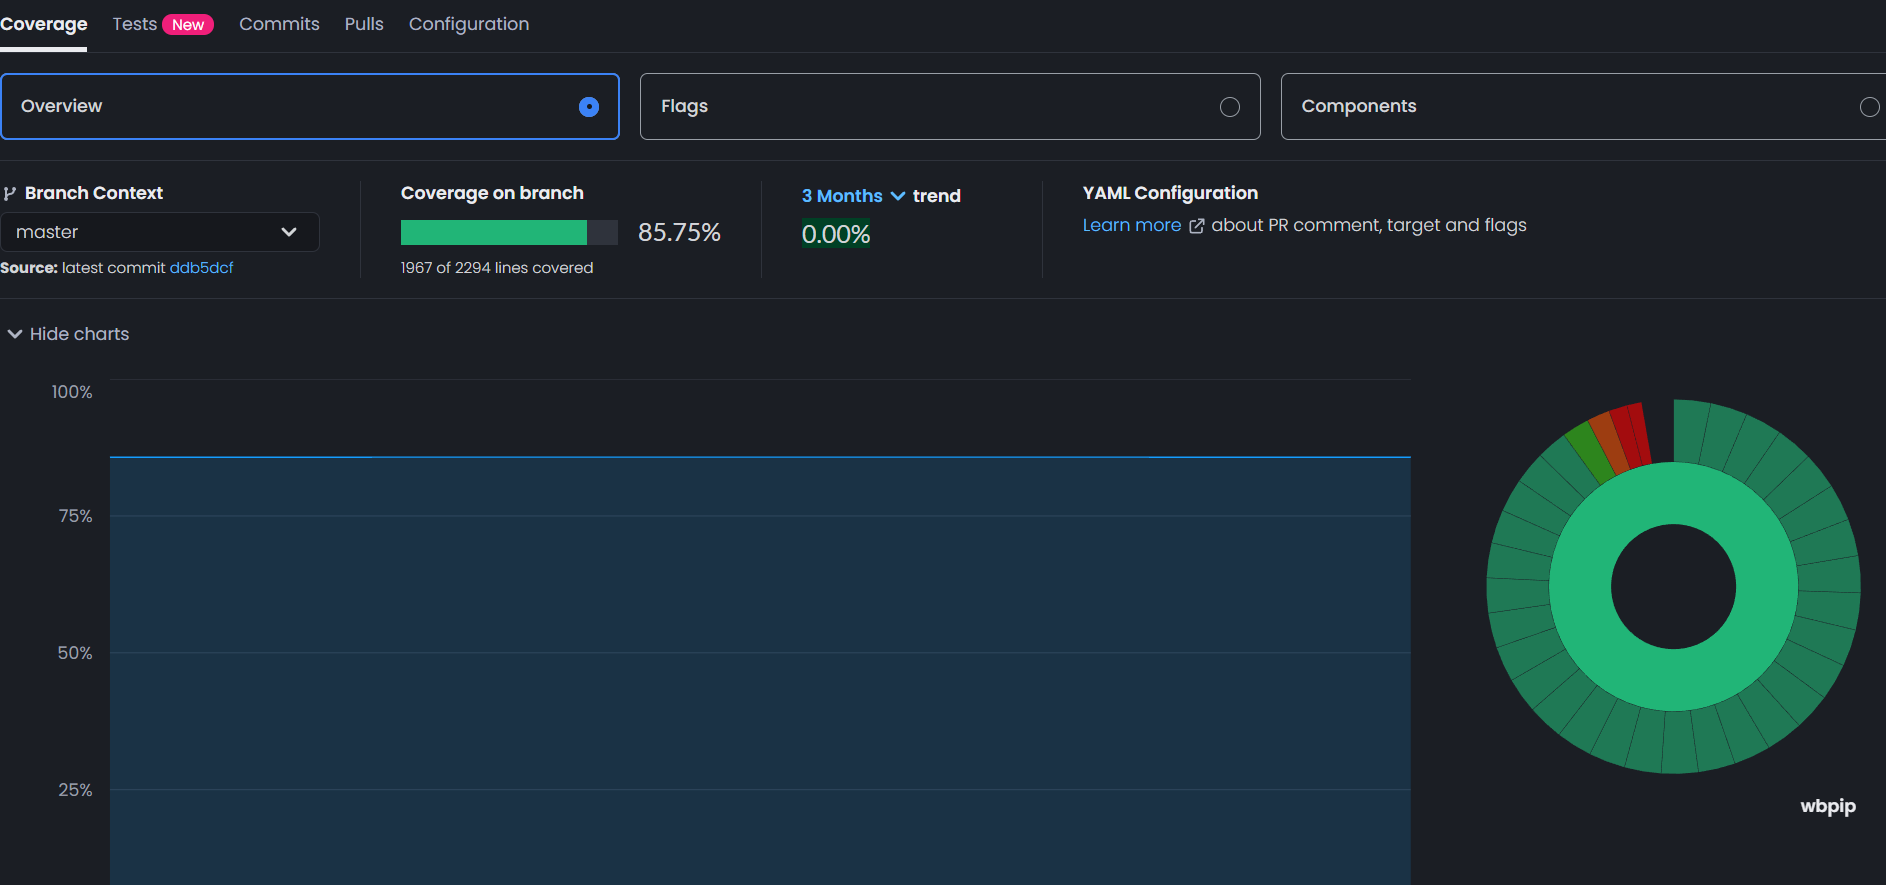
\includegraphics[keepaspectratio]{images/clipboard-2402093366.png}}
\item
  Every time a push or PR is made to \texttt{master} the dashboard will
  be updated with latest data.
\end{itemize}

\bookmarksetup{startatroot}

\chapter{Setting up Github Actions for Auto Deployment of Quarto
book}\label{setting-up-github-actions-for-auto-deployment-of-quarto-book}

\section{Introduction}\label{introduction-1}

One of the best parts of using Quarto for websites, blogs, or reports is
how easily it integrates with GitHub Pages. With a simple GitHub Actions
workflow, you can automatically render and publish your site every time
you update your repository. In this post we are going to learn how we
have enabled auto deployment for this quarto book.

\section{Workflow}\label{workflow}

This is the workflow that we are using in Github Actions . Let's look at
it one by one.

\begin{Shaded}
\begin{Highlighting}[]
\FunctionTok{on}\KeywordTok{:}
\AttributeTok{  }\FunctionTok{workflow\_dispatch}\KeywordTok{:}
\AttributeTok{  }\FunctionTok{push}\KeywordTok{:}
\AttributeTok{    }\FunctionTok{branches}\KeywordTok{:}\AttributeTok{ main}

\FunctionTok{name}\KeywordTok{:}\AttributeTok{ Quarto Publish}

\FunctionTok{jobs}\KeywordTok{:}
\AttributeTok{  }\FunctionTok{build{-}deploy}\KeywordTok{:}
\AttributeTok{    }\FunctionTok{runs{-}on}\KeywordTok{:}\AttributeTok{ ubuntu{-}latest}
\AttributeTok{    }\FunctionTok{permissions}\KeywordTok{:}
\AttributeTok{      }\FunctionTok{contents}\KeywordTok{:}\AttributeTok{ write}
\AttributeTok{    }\FunctionTok{steps}\KeywordTok{:}
\AttributeTok{      }\KeywordTok{{-}}\AttributeTok{ }\FunctionTok{name}\KeywordTok{:}\AttributeTok{ Check out repository}
\AttributeTok{        }\FunctionTok{uses}\KeywordTok{:}\AttributeTok{ actions/checkout@v4}

\AttributeTok{      }\KeywordTok{{-}}\AttributeTok{ }\FunctionTok{name}\KeywordTok{:}\AttributeTok{ Set up Quarto}
\AttributeTok{        }\FunctionTok{uses}\KeywordTok{:}\AttributeTok{ quarto{-}dev/quarto{-}actions/setup@v2}
\AttributeTok{        }\FunctionTok{env}\KeywordTok{:}
\AttributeTok{          }\FunctionTok{GH\_TOKEN}\KeywordTok{:}\AttributeTok{ $\{\{ secrets.GITHUB\_TOKEN \}\}}
\AttributeTok{        }\FunctionTok{with}\KeywordTok{:}
\AttributeTok{          }\FunctionTok{tinytex}\KeywordTok{:}\AttributeTok{ }\CharTok{true}
\AttributeTok{      }\KeywordTok{{-}}\AttributeTok{ }\FunctionTok{name}\KeywordTok{:}\AttributeTok{ Render and Publish}
\AttributeTok{        }\FunctionTok{uses}\KeywordTok{:}\AttributeTok{ quarto{-}dev/quarto{-}actions/publish@v2}
\AttributeTok{        }\FunctionTok{with}\KeywordTok{:}
\AttributeTok{          }\FunctionTok{target}\KeywordTok{:}\AttributeTok{ gh{-}pages}
\AttributeTok{        }\FunctionTok{env}\KeywordTok{:}
\AttributeTok{          }\FunctionTok{GITHUB\_TOKEN}\KeywordTok{:}\AttributeTok{ $\{\{ secrets.GITHUB\_TOKEN \}\}}
\end{Highlighting}
\end{Shaded}

\subsection{Triggering the Workflow}\label{triggering-the-workflow}

\begin{Shaded}
\begin{Highlighting}[]
\FunctionTok{on}\KeywordTok{:}
\AttributeTok{  }\FunctionTok{workflow\_dispatch}\KeywordTok{:}
\AttributeTok{  }\FunctionTok{push}\KeywordTok{:}
\AttributeTok{    }\FunctionTok{branches}\KeywordTok{:}\AttributeTok{ main}
\end{Highlighting}
\end{Shaded}

This tells GitHub Actions when to run the workflow. There are two
triggers here:

\begin{itemize}
\item
  \textbf{\texttt{push} to \texttt{main}} -- Any time you commit or
  merge changes into the \texttt{main} branch, the workflow runs
\item
  \textbf{\texttt{workflow\_dispatch}} -- Allows you to manually trigger
  the workflow from the GitHub Actions tab in your repository. This is
  useful when you want to force a rebuild and republish without
  committing new changes.
\end{itemize}

\subsection{Naming the workflow}\label{naming-the-workflow}

\begin{Shaded}
\begin{Highlighting}[]
\FunctionTok{name}\KeywordTok{:}\AttributeTok{ Quarto Publish}
\end{Highlighting}
\end{Shaded}

This gives the workflow a friendly name that will appear in the Actions
tab.

\subsection{Defining the job}\label{defining-the-job}

\begin{Shaded}
\begin{Highlighting}[]
\FunctionTok{jobs}\KeywordTok{:}
\AttributeTok{  }\FunctionTok{build{-}deploy}\KeywordTok{:}
\AttributeTok{    }\FunctionTok{runs{-}on}\KeywordTok{:}\AttributeTok{ ubuntu{-}latest}
\AttributeTok{    }\FunctionTok{permissions}\KeywordTok{:}
\AttributeTok{      }\FunctionTok{contents}\KeywordTok{:}\AttributeTok{ write}
\end{Highlighting}
\end{Shaded}

Here we're defining a single job called \texttt{build-deploy}.

\begin{itemize}
\item
  \textbf{\texttt{runs-on:\ ubuntu-latest}} -- The job will run inside
  an Ubuntu-based virtual machine provided by GitHub.
\item
  \textbf{\texttt{permissions:\ contents:\ write}} -- The workflow needs
  permission to write to the repository (required for publishing to the
  \texttt{gh-pages} branch).
\end{itemize}

\subsection{The Steps}\label{the-steps}

\subsubsection{1. Check out the
repository}\label{check-out-the-repository}

\begin{Shaded}
\begin{Highlighting}[]
\KeywordTok{{-}}\AttributeTok{ }\FunctionTok{name}\KeywordTok{:}\AttributeTok{ Check out repository}
\AttributeTok{  }\FunctionTok{uses}\KeywordTok{:}\AttributeTok{ actions/checkout@v4}
\end{Highlighting}
\end{Shaded}

This makes your repository's files available in the workflow environment
so Quarto can render your project.

\subsubsection{2. Set up Quarto}\label{set-up-quarto}

\begin{Shaded}
\begin{Highlighting}[]
\KeywordTok{{-}}\AttributeTok{ }\FunctionTok{name}\KeywordTok{:}\AttributeTok{ Set up Quarto}
\AttributeTok{  }\FunctionTok{uses}\KeywordTok{:}\AttributeTok{ quarto{-}dev/quarto{-}actions/setup@v2}
\AttributeTok{  }\FunctionTok{env}\KeywordTok{:}
\AttributeTok{    }\FunctionTok{GH\_TOKEN}\KeywordTok{:}\AttributeTok{ $\{\{ secrets.GITHUB\_TOKEN \}\}}
\AttributeTok{  }\FunctionTok{with}\KeywordTok{:}
\AttributeTok{    }\FunctionTok{tinytex}\KeywordTok{:}\AttributeTok{ }\CharTok{true}
\end{Highlighting}
\end{Shaded}

This installs Quarto in the workflow environment. The
\texttt{tinytex:\ true} option ensures LaTeX support is available for
rendering PDFs. The \texttt{GH\_TOKEN} is github token repository secret
that is added in Repo settings -\textgreater{} Secrets and Variables
-\textgreater{} Actions . It is used for authentication when publishing.

\subsubsection{3. Render and Publish}\label{render-and-publish}

\begin{Shaded}
\begin{Highlighting}[]
\KeywordTok{{-}}\AttributeTok{ }\FunctionTok{name}\KeywordTok{:}\AttributeTok{ Render and Publish}
\AttributeTok{  }\FunctionTok{uses}\KeywordTok{:}\AttributeTok{ quarto{-}dev/quarto{-}actions/publish@v2}
\AttributeTok{  }\FunctionTok{with}\KeywordTok{:}
\AttributeTok{    }\FunctionTok{target}\KeywordTok{:}\AttributeTok{ gh{-}pages}
\AttributeTok{  }\FunctionTok{env}\KeywordTok{:}
\AttributeTok{    }\FunctionTok{GITHUB\_TOKEN}\KeywordTok{:}\AttributeTok{ $\{\{ secrets.GITHUB\_TOKEN \}\}}
\end{Highlighting}
\end{Shaded}

This step does two things:

\begin{enumerate}
\def\labelenumi{\arabic{enumi}.}
\item
  \textbf{Renders} your Quarto project (turns \texttt{.qmd} files into
  HTML, PDF, or other output formats).
\item
  \textbf{Publishes} the output to the \texttt{gh-pages} branch, which
  GitHub Pages uses to serve your site. The \texttt{target:\ gh-pages}
  option ensures everything is pushed to the right branch.
\end{enumerate}

\section{\texorpdfstring{Don't ignore the \texttt{.gitignore}
file}{Don't ignore the .gitignore file}}\label{dont-ignore-the-.gitignore-file}

Make sure that your \texttt{.gitignore} file excludes \texttt{\_book},
\texttt{\_site} folders. These are the folders where Quarto renders
HTML/PDF files when testing them locally. These files should not be
tracked since Github Actions will build them with our auto deployment
process.

\section{Conclusion :}\label{conclusion}

With this workflow in place, the Quarto book will automatically rebuild
and deploy whenever a push is made to the \texttt{main} branch or
whenever we manually trigger the workflow. No more running commands
locally or remembering to push generated files.

This is a clean, reproducible, and automated way to publish your Quarto
projects using GitHub Pages. As a side not \texttt{usethis} package has
a lot of good utility functions that helps you to set up similar
workflow. You may explore using them. A good starting point is
\texttt{usethis::use\_github\_action("render-quarto")}.

For reference the Quarto book is published
\href{https://gpid-wb.github.io/Pip-Technical-Guidelines/}{here}.

\bookmarksetup{startatroot}

\chapter{Improve Efficiency of a WB
Laptop}\label{improve-efficiency-of-a-wb-laptop}

There are a few things you can do to improve the efficiency of a WB
laptop. These tips won't make your laptop \emph{fast}, but they will
help optimize performance and make it feel more responsive.

\begin{center}\rule{0.5\linewidth}{0.5pt}\end{center}

\section{Modify System Properties for
Performance}\label{modify-system-properties-for-performance}

\begin{enumerate}
\def\labelenumi{\arabic{enumi}.}
\item
  Open the Windows menu, type \textbf{Run}, and click on the \emph{Run}
  app.\\
  \pandocbounded{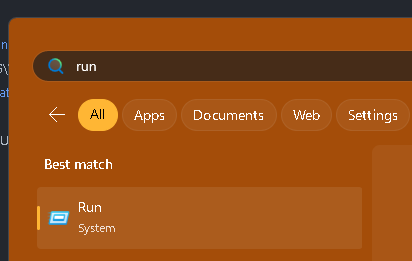
\includegraphics[keepaspectratio]{images/Increase_performance_WB_laptop/run.png}}
\item
  In the Run app, type the following command and hit \textbf{Enter}:
\end{enumerate}

\begin{Shaded}
\begin{Highlighting}[]
\NormalTok{   systempropertiesperformance.exe}
\end{Highlighting}
\end{Shaded}

\pandocbounded{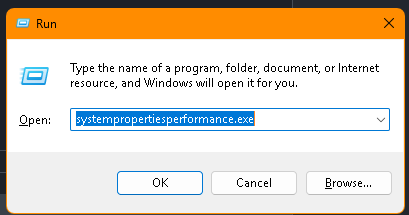
\includegraphics[keepaspectratio]{images/Increase_performance_WB_laptop/run_box.png}}

\begin{enumerate}
\def\labelenumi{\arabic{enumi}.}
\setcounter{enumi}{2}
\item
  In the \emph{Performance Options} window, select the \textbf{Visual
  Effects} tab.

  \begin{itemize}
  \tightlist
  \item
    Click on \textbf{Adjust for best performance}.
  \item
    Make sure all the checkboxes are unchecked.
  \item
    Click \textbf{Apply} and then \textbf{OK}.
  \end{itemize}

  \pandocbounded{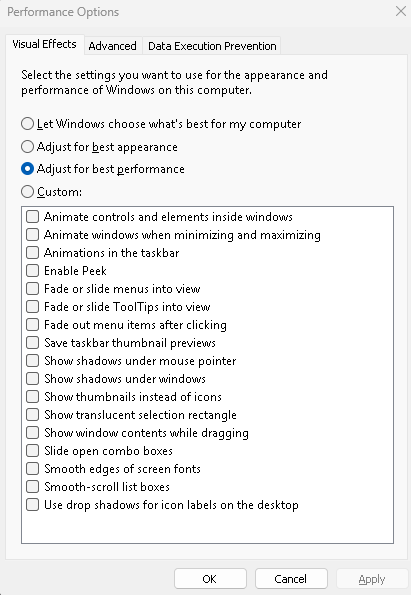
\includegraphics[keepaspectratio]{images/Increase_performance_WB_laptop/performance_options.png}}
\end{enumerate}

\begin{tcolorbox}[enhanced jigsaw, leftrule=.75mm, left=2mm, title=\textcolor{quarto-callout-warning-color}{\faExclamationTriangle}\hspace{0.5em}{Warning}, arc=.35mm, opacityback=0, colback=white, coltitle=black, colframe=quarto-callout-warning-color-frame, bottomrule=.15mm, colbacktitle=quarto-callout-warning-color!10!white, breakable, toptitle=1mm, rightrule=.15mm, bottomtitle=1mm, opacitybacktitle=0.6, toprule=.15mm, titlerule=0mm]

\textbf{Note:} This may affect the appearance of your system, since many
visual effects will be disabled.

\end{tcolorbox}

\begin{center}\rule{0.5\linewidth}{0.5pt}\end{center}

\section{Battery Settings}\label{battery-settings}

\begin{enumerate}
\def\labelenumi{\arabic{enumi}.}
\item
  Open \textbf{Battery Settings}.
  \pandocbounded{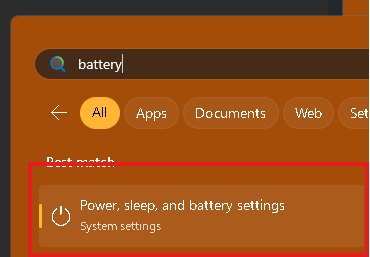
\includegraphics[keepaspectratio]{images/Increase_performance_WB_laptop/battery_settings.png}}
\item
  Set the battery mode to \textbf{Best performance}.
  \pandocbounded{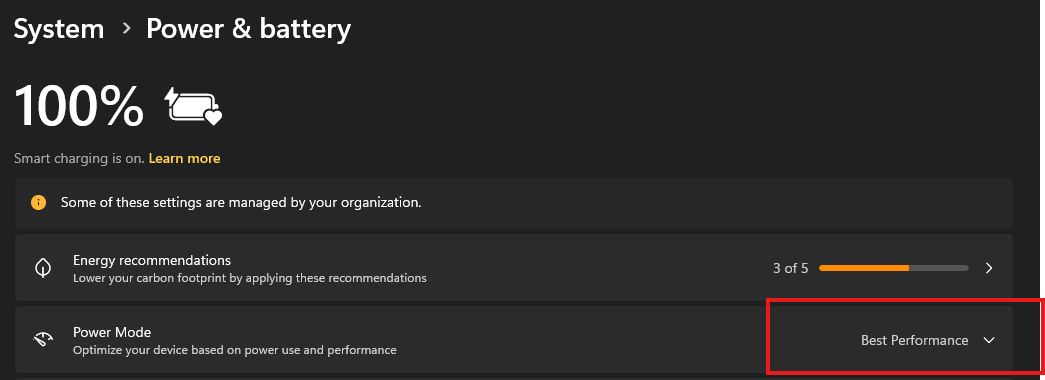
\includegraphics[keepaspectratio]{images/Increase_performance_WB_laptop/battery_best_performance.png}}
\end{enumerate}

\begin{center}\rule{0.5\linewidth}{0.5pt}\end{center}

\section{Google Chrome Settings}\label{google-chrome-settings}

\begin{enumerate}
\def\labelenumi{\arabic{enumi}.}
\item
  In Google Chrome, type the following in the address bar:

\begin{Shaded}
\begin{Highlighting}[]
\NormalTok{chrome://settings/performance}
\end{Highlighting}
\end{Shaded}
\item
  Under the \textbf{Memory} section, select \textbf{Maximum}.
  \pandocbounded{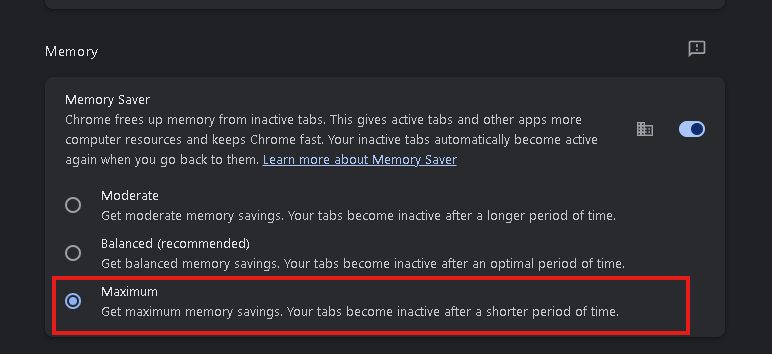
\includegraphics[keepaspectratio]{images/Increase_performance_WB_laptop/google_max_performance.png}}
\end{enumerate}

\bookmarksetup{startatroot}

\chapter{Summary}\label{summary}

\bookmarksetup{startatroot}

\chapter*{References}\label{references}
\addcontentsline{toc}{chapter}{References}

\markboth{References}{References}




\end{document}
